\documentclass{article}[18pt]
\ProvidesPackage{format}
%Page setup
\usepackage[utf8]{inputenc}
\usepackage[margin=0.7in]{geometry}
\usepackage{parselines} 
\usepackage[english]{babel}
\usepackage{fancyhdr}
\usepackage{titlesec}
\hyphenpenalty=10000

\pagestyle{fancy}
\fancyhf{}
\rhead{Sam Robbins}
\rfoot{Page \thepage}

%Characters
\usepackage{amsmath}
\usepackage{amssymb}
\usepackage{gensymb}
\newcommand{\R}{\mathbb{R}}

%Diagrams
\usepackage{pgfplots}
\usepackage{graphicx}
\usepackage{tabularx}
\usepackage{relsize}
\pgfplotsset{width=10cm,compat=1.9}
\usepackage{float}

%Length Setting
\titlespacing\section{0pt}{14pt plus 4pt minus 2pt}{0pt plus 2pt minus 2pt}
\newlength\tindent
\setlength{\tindent}{\parindent}
\setlength{\parindent}{0pt}
\renewcommand{\indent}{\hspace*{\tindent}}

%Programming Font
\usepackage{courier}
\usepackage{listings}
\usepackage{pxfonts}

%Lists
\usepackage{enumerate}
\usepackage{enumitem}

% Networks Macro
\usepackage{tikz}


% Commands for files converted using pandoc
\providecommand{\tightlist}{%
	\setlength{\itemsep}{0pt}\setlength{\parskip}{0pt}}
\usepackage{hyperref}

% Get nice commands for floor and ceil
\usepackage{mathtools}
\DeclarePairedDelimiter{\ceil}{\lceil}{\rceil}
\DeclarePairedDelimiter{\floor}{\lfloor}{\rfloor}

% Allow itemize to go up to 20 levels deep (just change the number if you need more you madman)
\usepackage{enumitem}
\setlistdepth{20}
\renewlist{itemize}{itemize}{20}

% initially, use dots for all levels
\setlist[itemize]{label=$\cdot$}

% customize the first 3 levels
\setlist[itemize,1]{label=\textbullet}
\setlist[itemize,2]{label=--}
\setlist[itemize,3]{label=*}

% Definition and Important Stuff
% Important stuff
\usepackage[framemethod=TikZ]{mdframed}

\newcounter{theo}[section]\setcounter{theo}{0}
\renewcommand{\thetheo}{\arabic{section}.\arabic{theo}}
\newenvironment{important}[1][]{%
	\refstepcounter{theo}%
	\ifstrempty{#1}%
	{\mdfsetup{%
			frametitle={%
				\tikz[baseline=(current bounding box.east),outer sep=0pt]
				\node[anchor=east,rectangle,fill=red!50]
				{\strut Important};}}
	}%
	{\mdfsetup{%
			frametitle={%
				\tikz[baseline=(current bounding box.east),outer sep=0pt]
				\node[anchor=east,rectangle,fill=red!50]
				{\strut Important:~#1};}}%
	}%
	\mdfsetup{innertopmargin=10pt,linecolor=red!50,%
		linewidth=2pt,topline=true,%
		frametitleaboveskip=\dimexpr-\ht\strutbox\relax
	}
	\begin{mdframed}[]\relax%
		\centering
		}{\end{mdframed}}



\newcounter{lem}[section]\setcounter{lem}{0}
\renewcommand{\thelem}{\arabic{section}.\arabic{lem}}
\newenvironment{defin}[1][]{%
	\refstepcounter{lem}%
	\ifstrempty{#1}%
	{\mdfsetup{%
			frametitle={%
				\tikz[baseline=(current bounding box.east),outer sep=0pt]
				\node[anchor=east,rectangle,fill=blue!20]
				{\strut Definition};}}
	}%
	{\mdfsetup{%
			frametitle={%
				\tikz[baseline=(current bounding box.east),outer sep=0pt]
				\node[anchor=east,rectangle,fill=blue!20]
				{\strut Definition:~#1};}}%
	}%
	\mdfsetup{innertopmargin=10pt,linecolor=blue!20,%
		linewidth=2pt,topline=true,%
		frametitleaboveskip=\dimexpr-\ht\strutbox\relax
	}
	\begin{mdframed}[]\relax%
		\centering
		}{\end{mdframed}}
\lhead{Software Methodologies - Image Processing}


\begin{document}
\begin{center}
\underline{\huge Colour spaces and adding colour to grayscale images}
\end{center}
\section{RGB Colour Space}
Colours represented as R,G,B intensities.\\
\\
The space is modelled geometrically by a cube with axes R,G and B\\
\\
RGB is used as it is based on the human perception of the visible spectrum - the human eye has R, G and B receptors with different sensitivity at different wavelengths
{\renewcommand{\arraystretch}{2}
\section{HSV colour space}
\begin{tabularx}{\textwidth}{|X|X|X|}
\hline
H(ue)& Specifies the dominant wavelength & $0 \rightarrow 360^\circ$\\
\hline
S(aturation)& High values correspond to vibrant pure colours& $0\rightarrow 1$\\
\hline
V(alue)&Brightness of colour& $0\rightarrow 1$\\
\hline
\end{tabularx}}
\subsection{The geometry of the HSV space}
The hue is mapped cyclically, so red corresponds to both 0 and 360, so the HSV space can be modelled by a cylinder\\
\\
When we map the RGB cube onto the HSV cylinder we get a subset of this cylinder in the shape of a pyramid with hexagonal base, which in turn gives rise to the cone model
\subsection{Thresholding}
Thresholding produces a binary image from a grayscale image\\
\\
Easier to colour threshold in HSV space than RGB
\begin{definition}[Colour slicing]
	A portion of the Hue colour channel (range of wavalengths) can be isolated. For better results, also use S and V in conjunctoon
\end{definition}
Isolate objects by colour:
\begin{itemize}
	\item Use an upper and lower threshold on the Hue channel to isolate by colour
	\item Use a threshold on the Saturation channel to isolate pure colours
	\item Combine the two outputs with logical AND
\end{itemize}
\textbf{Specular highlights}
\begin{itemize}
	\item RGB: very different position in space to original colour
	\item HSV: similar position in Hue as specular present in Value
\end{itemize}
\textbf{Shadows}:
\begin{itemize}
	\item HSV: isolated in the Saturation/Value components
\end{itemize}
\section{CMY colour space}
CMY is a subtractive colour model based on mixing pigments of Cyan, Magenta and Yellow to create other colours.\\
\\
The colours that are seen are part of the visible spectrum that is not absorbed by the pigments\\
\\
The CMY colour space can be modelled by a cube
\begin{center}
	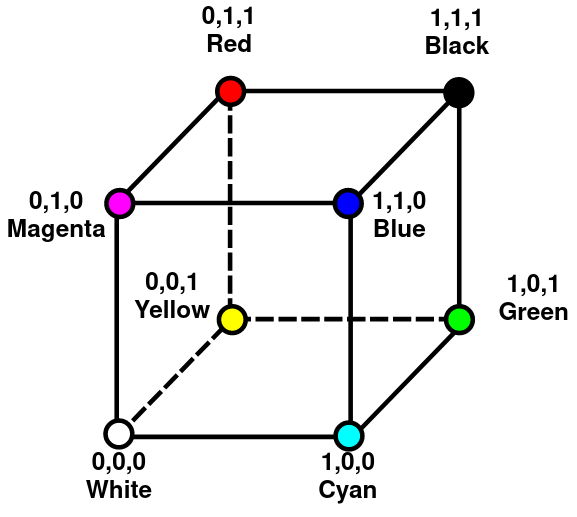
\includegraphics[scale=0.7]{CMY}
\end{center}
\section{CMYK colour space}
CMYK is an extension of CMY, with the addition of K, which is pure black and absorbs all light in the visible spectrum.\\
\\
In CMY the black can also be generated by mixing all the colours, but due to pigment imperfections, is not as dark as black ink. For this reason CMYK has better contrast.
\section{L*a*b colour space}
L*a*b is a perceptually uniform colour space. Changes in the L*a*b values are commensurate with changes in human perception of colour.\\
\\
L*a*b colours are specified through properties of light (distributions of wavelengths) and thus, unlike RGB, do not depend on the device that generates them\\
Extends RGB and CMYK. Covers all visible colours and its parameter space can specify non visible colours.
\section{Adding colour to grayscale images}
\subsection{Intensity Slicing}
Consider the intensity levels
$$l_0<l_1<l_2<...<l_M$$
where $l_0$ corresponds to black and $l_M$ to white\\
\\
We use the M colours
$$c_0,c_1,c_2,...,c_{M-1}$$
and a pixel with intensity s is assigned the colour $c_k$ if
$$l_k\leqslant s<l_{k-1}$$
while $l_M$ is assigned $c_{M-1}$
\subsection{Transfer functions}
More general technique for colour mapping
\begin{itemize}
	\item Scalar value s; colour value c
	\item Colour transfer function: $f(s)=c$
\end{itemize}
Any functional expression can map s into values for the colour components $c_1,c_2,c_3$





\end{document}